%*************************************************************
\chapter{Kollaboratives Design}\label{ch:kollaborativesDesign}
%*************************************************************

Kollaborative Aktivitäten sind ein wichtiger Anwendungsbereich für elektronische Technologien \citep{Kvan:2000}. Designer arbeiten immer häufiger nicht mehr alleine für sich, sondern mit anderen Designern, aber auch Leuten aus anderen Disziplinen zusammen. Da komplexe Probleme mehr Expertise und Wissen erfordern, als eine einzelne Person haben kann, sind Teilnahme, Kommunikation und Kollaboration seitens aller involvierten Akteure notwendig. Die intellektuelle, kulturelle und soziale Vielfalt, die dem Projekt dadurch zugutekommt, ist eine wichtige Quelle für soziale Kreativität \citep{Fischer:2005}. 

\medskip Für das Verständnis von kollaborativem Design ist es wichtig, die Bedeutung von Kollaboration zu erörtern. Betrachten wir dazu die verschiedenen Aktivitäten, die gemeinhin unter dem Begriff Kollaboration zusammengefasst werden. Zur Lösung von gegebenen Problemen, beispielsweise dem Design eines neuen Produkts, bilden Individuen Teams und Gruppen, um vom sogenannten >>process gain<< \citep{steiner:1972} zu profitieren. Von kollaborativem Erfolg kann dann gesprochen werden, wenn die Gruppe etwas erreicht, das ihre  Mitglieder alleine nicht hätten erreichen können \citep{Kvan:2000}. Kollaboration kann als gemeinsames Lösen von Problemen verstanden werden: Individuen haben ein oder mehrere gemeinsame Ziele und arbeiten zusammen, um befriedigende Lösungen zu finden. Thomas Kvan definiert den Begriff Kollaboration durch Bezugnahme auf auf das Oxford Englischwörterbuch:

\begin{quote} 
	>>Indeed, the Oxford English Dictionary de- fines collaborate as ‘‘to co-operate, especially in literary, artistic or scientific work’’, deriving from the Latin words \emph{col labore}, to work along side one another.<< \citep{Kvan:2000} 
\end{quote} 

Weiters schreibt er, dass kollaboratives Design eine weitaus anspruchsvollere Aktivität ist, als einfach nur ein Projekt in einem Team abzuschließen. Es muss ein gemeinsames, ganzheitliches und kreatives Resultat produziert, nicht bloß eine gewisse Arbeit erledigt werden \citep{Kvan:2000}.

Viele Arten von Design können nicht von einem einzelnen Designer gehandhabt werden. Im Bereich Architektur arbeiten beispielsweise sehr viele Leute aus verschiedenen Disziplinen zusammen, um ein Gebäude zu entwerfen. 

HIER NOCH WEITER SCHREIBEN: COLLABORATIVE DESIGN WHAT IS IT?

\section{Soziale Aspekte \& Probleme} 

Kollaboratives Design von mehreren Personen aus verschiedenen beruflichen Disziplinen birgt sehr viele und komplexe soziale Aspekte. Jede dieser Personen hat einen eigenen Charakter, verschiedene kulturelle, soziale und politische Ansichten und vor allem eigene Interessen und Sichtweisen.

\autoref{fig:kilkerTree} zeigt den sogenannten >>Tree Swing<<\footnote{zu Deutsch: Baumschaukel} Sketch, der auf witzige Weise die Problematik von kollaborativem Design aufzeigt. Man sieht darin die verschiedenen Visionen einer Baumschaukel der jeweiligen Teammitglieder. Jede einzelne Darstellung der Schaukel stereotypisiert eine ins Projekt involvierte Rolle \citep{Kilker:1999}.

\medskip Designprojekte im technologischen Bereich umfassen immer mehr Teammitglieder aus unterschiedlichen Berufsgruppen. Egal ob diese Personen in einem Meeting zusammensitzen oder ihre Arbeit via Videokonferenz erledigen, sie alle haben verschiedne Perspektiven auf das Projekt, die Anforderungen und die Lösung. Jeder muss seine eigene Sichtweisen argumentieren und versuchen so gut wie möglich durchzusetzen, ähnlich dem Sketch in \autoref{fig:kilkerTree}. Julian Kilker bezeichnet diese verschiedenen Rollen als >>design identities<<\footnote{zu Deutsch: Designidentität}. Jede dieser >>design identities<< hat eine eigene Meinung, eigene Standpunkte und eine eigene Einstellung gegenüber Technologie und Design. All diese Faktoren beeinflussen das Design, den Prozess und das Endprodukt der Projektarbeit \citep{Kilker:1999}.

\begin{figure}
	{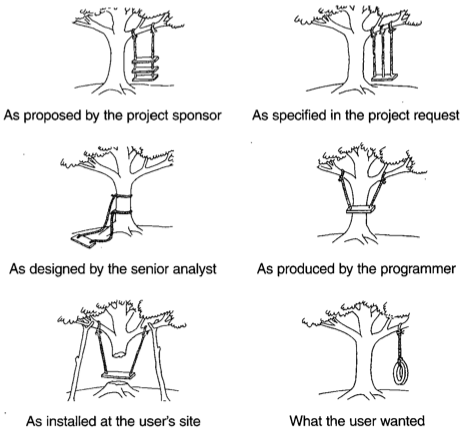
\includegraphics[width=1\linewidth]{gfx/kilkerTreeSwing}}
\caption[Tree Swing Sketch]{Der >>Tree Swing<< (Baumschaukel) Sketch zeigt die Fallen, in die man bei kollaborativem Design laufen kann. Wenn jeder eine andere Vorstellung vom Produkt hat, dann leidet das Endresultat. \citep{Kilker:1999}}\label{fig:kilkerTree}
\end{figure}

\medskip Die Theorie der sozialen Identität ist eine sozialpsychologische Perspektive, die erläutert, wie Menschen soziale Identitäten (beispielsweise >>Entwickler<<, >>Manager<< oder >>Programmierer<<) annehmen, halten und verwenden \citep{Hogg:1988}.

Aufbauend auf Sherifs Untersuchungen der realistischen Konflikttheorie \citep{Sherif:1966}, ist die Theorie der sozialen Identität nützlich für die Erforschung der Art und Weise, wie Individuen in Gruppen zusammenarbeiten \citep{Kilker:1999}. Personen sind Teil einer sozialen Gruppe, wenn sie eine gemeinsame Definition ihrer selbst als Teil dieser Gruppe vertreten \citep{Hogg:1988}.

Sherif hat Konflikte in Gruppen und Teams ausgiebig untersucht. Dabei hat er für seine Zwecke die Testpersonen so in Gruppen aufgeteilt, dass ein möglichst kompetitives Klima innerhalb des jeweiligen Teams entstand \citep{Sherif:1966}. Die Theorie der sozialen Identität fokussiert im Gegensatz zu diesen designierten Teams auf möglichst realistische Gruppenkonstellationen.

\medskip Idealisierte soziale Identitäten spielen bei Interaktionen innerhalb einer Gruppe eine wichtige Rolle. Menschen brauchen sie, um sich selbst und andere zu definieren und Vergleiche herzustellen. Jeder hat ein stereotypes Bild der einzelnen involvierten Berufsdisziplinen im Kopf, basierend auf Bildung und Erfahrung. Der Theorie der sozialen Identität zufolge, betonen Leute im eigenen Team Ähnlichkeiten zwischen sich und den Kollegen, gegenüber anderen Gruppen heben sie jedoch Unterschiede hervor. Generell kommen stereotype Sichtweisen eher in multidisziplinären (heterogenen) Teams zum Vorschein, als in homogenen Konstellationen.

\medskip Im sozialen Wettbewerb tendieren soziale Identitäten zur Polarisation. Die Individuen ordnen sich und den anderen eine gewisse Identität und dessen Ideale zu und kategorisieren damit jeden in der Gruppe. Solche polarisierenden Identitäten sind beispielsweise Liberale oder Konservative in politischer Hinsicht, Vertreter von qualitativen oder quantitativen Methoden in wissenschaftlicher Hinsicht oder die stereotypischen Interpretationen von PC oder Mac Benutzern.

Stereotype sind von Natur aus simplifiziert und stilisiert. Kein Mensch entspricht genau so einem verzerrten Bild, denn jeder hat Ansichten, Ideale und Eigenschaften, die sich davon unterscheiden. 

\medskip Obwohl es im Bereich Design viele unterschiedliche soziale Identitäten gibt, wollen wir uns im Folgenden auf zwei typische Identitäten konzentrieren: eine vertritt Ansichten und Methoden, die technologiezentriert sind und die andere vertritt sozialzentrierte Ansichten und Methoden. Wir prüfen die Kollaboration zwischen diesen zwei Charakteren und die damit verbundenen Implikationen \citep{Kilker:1999}.

Die technologiezentrierte Identität bevorzugt ein gut geplantes, systematisches und lineares Design, das Pahl und Beitz als >>systematischen Ansatz<< bezeichnen \citep{Pahl:1988}, während die sozialzentrierte Identität benutzerzentriertes und partizipatives Design sowie eine iterative Vorgehensweise vorzieht.

\autoref{tab:kilkerIdeals} zeigt die unterschiedlichen, polarisierenden Ideale dieser beiden Designidentitäten nach Kilker \citep{Kilker:1999}. Donald Norman nennt diese auseinander laufenden Perspektiven >>menschenzentriert<< und >>maschinenzentriert<<. Erstere ordnet den Menschen der Maschine über, denn er ist der Maschine durch Kreativität, Einfallsreichtum und Flexibilität überlegen. Computer hingegen sind dumm, einfallslos und starr. Die maschinenzentrierte Perspektive sieht den Menschen dagegen als unorganisiert, emotional und unlogisch, während Maschinen als geordnet, objektiv und logisch betrachtet werden \citep{Norman:1994}. 

\begin{table}
    \myfloatalign
\begin{tabularx}{\textwidth}{p{2.4cm}XX}
    \toprule
	    \tableheadline{Faktor} & \tableheadline{TZI} & \tableheadline{SZI}
	       	\\ \midrule
	
			\small{
				Charakteristiken guten Designs
			} & 
			\small{
				Fokus auf technologische Charakteristiken: Effiziente >>clevere<< Lösung, geringer Instandhaltungsaufwand. Das beste Design kann quantitativ ermittelt werden und das Ziel ist es, dieses zu implementieren
			} & 
			\small{
				Fokus auf soziale Charakteristiken: Funktioniert in der gegebenen sozialen Umgebung und befriedigt die Bedürfnisse der Benutzer. Es gibt mehrere Perspektiven von gutem Design und das Ziel ist es, die beste Kombination zu finden.
			} \\
			\hline %------------------------------------------------------------
			\small{
				Designprozess
			} & 
			\small{
				Systemorientiert, basierend auf Spezifikationen
			} & 
			\small{
				Iterativ, benutzerorientiert. Kollaboration verbessert Design.
			} \\
			\hline %------------------------------------------------------------
			\small{
				Verantwortung der Designer
			} & 
			\small{
				Designer sind nicht verantwortlich für soziale Verwendung von Technologie, die Verantwortung liegt beim Benutzer.
			} & 
			\small{
				Designer sollen den sozialen Kontext der Technologie berücksichtigen.
			} \\
			\hline %------------------------------------------------------------
			\small{
				Die Rolle von Evaluierung in Design
			} & 
			\small{
				Quantitativ: gibt an, ob die Implementierung die Anforderungen der Spezifikation erfüllt. Benutzer gehen nicht rein logisch vor, ihre Evaluierung ist oft widersprüchlich und bringt wenig.
			} & 
			\small{
				Qualitativ und ethnographisch: zeigt Diskrepanzen zwischen Spezifikation und Bedürfnissen der Nutzer auf. Die Benutzer haben höchste Priorität und sollten deshalb in den Designprozess einbezogen werden.
			} \\
			\hline %------------------------------------------------------------
			\small{
				Wie wird das andere Ideal wahrgenommen?
			} & 
			\small{
				Sozialzentrierten Idealen fehlt es an konkreten Zielen. Befürworter verlangen oft substanzielle Designänderungen aufgrund von Trivialitäten.
			} & 
			\small{
				Technologiezentrierte Ideale sind starr und unflexibel. Befürworter sind zwar technisch kompetent, weigern sich aber, soziale Aspekte zu berücksichtigen.
			}
			\\ \bottomrule
\end{tabularx}
  \caption[Polarisierende Designideale]{Die unterschiedlichen Designideale von technologiezentrierten und sozialzentrierten Identitäten \citep{Kilker:1999}. \\TZI = Technologiezentriertes Ideal \\SZI = Sozialzentriertes Ideal}
  \label{tab:kilkerIdeals}
\end{table}

\medskip Neben der stereotypischen Sichtweise der Kollegen im Projekt, hat auch jeder Designer ein stereotypisches Bild vom designierten Endbenutzer. Problematisch ist jedoch bereits die Begrifflichkeit >>der (End)benutzer<<, da Technologien von sehr vielen und sehr unterschiedlichen Individuen aus verschiedenen Kontexten benutzt werden \citep{Agre:1995}. Daher muss der Begriff >>Benutzer<< explizit und implizit während des Designprozesses erörtert und ein authentisches Bild vom tatsächlichen Endbenutzer geschaffen werden. Designer können dies direkt durch Diskussion mit und Observation von potenziellen Nutzern oder indirekt und hypothetisch durch Stereotypisierung von Szenarios und Fallstudien erreichen.

\medskip Eine hypothetische Benutzergruppe wäre beispielsweise der >>naive user<<, der laut Annahme der Technologie komplett fremd ist. Technologiezentriertes Design würde davon ausgehen, dass dieser Benutzer in der selben Welt wie der Programmierer lebt und dass rationale und formale Methoden eingesetzt werden können, um die Interaktionen zwischen diesem Menschen und der Maschine zu modellieren. Das Gegenlager, sozialzentriertes Design, würde mit der Annahme starten, technische Systeme könnten nicht ohne ein umfassendes Verständnis des sozialen Kontexts entwickelt werden und die Zielgruppe müsste aktiv auf die neue Technologie vorbereitet werden.

\medskip Soziale Identitäten sind in zweierlei Weisen eine Herausforderung bei der Kollaboration in einem Team: zum einen ist es für die involvierten Personen schwierig, ihre unterschiedlichen Perspektiven und Meinungen zu vereinbaren, und zum anderen hat auch jeder der Beteiligten eine andere Vorstellung davon, wie der Designprozess und die Kollaboration selbst ablaufen sollen.

Jeder Mensch ist immer Teil von mehreren sozialen Gruppen. In einem kollaborativen Designkontext ist jeder ein Teil des Projektteams und zusätzlich noch Teil seiner Berufsgruppe und den damit verbundenen sozialen Kontext. Der Zwiespalt zwischen diesen beiden Gruppen kann dazu führen, dass die Qualität der Zusammenarbeit leidet. Wenn Teammitglieder zu sehr die Rolle ihrer Berufsgruppe einnehmen, kann das in festgefahrenen Diskussionen resultieren \citep{Kilker:1999}. Wird hingegen die Identität als Teammitglied zu sehr in den Vordergrund gerückt, kann dies dazu führen, dass die eigene Perspektive nicht mehr genügend eingebracht und dadurch wertvoller Input verloren geht \citep{Irving:1982}.

Sherif hat durch seine Forschung herausgefunden, dass die Kollaboration zwischen polarisierenden Identitäten durch die Einführung eines gemeinsamen Gegners, oder schärfer gesagt, durch die Einführung eines Feindes angekurbelt werden kann. Besser ist es hingegen, übergeordnete Ziele für die Gruppe einzuführen, deren Erreichung für das Team äußerst reizvoll ist und die für das einzeln Individuum absolut unerreichbar sind \citep{Sherif:1966}.

Viele Mitglieder in Designteams sind in kollaborativem Arbeiten ungeübt. Dieses Problem rührt daher, dass technische Ausbildungen darauf abzielen, optimale Lösungen zu finden, anstatt auch Kompromisse und Mittelwege in Betracht zu ziehen. Sozialzentrale Ausbildungen lehren hier eine andere Vorgangsweise. Sie propagieren in kollaborativer Arbeit auch zu diskutieren und zu verhandeln, das technologiezentrierte Lager empfindet diese Methoden hingegen als ineffektiv. Wir wollen dazu einen beispielhaften Kommentar aus einer Online-Gruppendiskussion über Hypertextstandards\footnote{Unter Hypertext wird in der Regel ein Text mit aktivierbaren Elementen verstanden, die im einfachsten Fall dazu dienen, direkt zu anderen Stellen im Text oder zu anderen Texten zu springen} betrachten, in dem er sich für seinen harschen Tonfall in einer vorhergehenden Aussage rechtfertigt:

\begin{quote}
	>>I try to discourage what I see as bad practice, I'm stronger about it here because I think we're alle technical people, I know as an engineer I much prefer direct talk to soft sell. And my experience is most engineers aren't overly sensitive - they can take heat as well as give it without making it a personal issue.<<\footnote{zu Deutsch: >>Ich versuche immer von schlechten Methoden abzuraten. Ich tue das in dieser direkten Form, weil ich denke wir sind hier Techniker unter uns. Als Ingenieur bevorzuge ich, Dinge direkt und konkret anzusprechen und meine Erfahrung hat mir gezeigt, dass die meisten Ingenieure nicht sonderlich zimperlich oder sensibel sind. Sie können hitzige Diskussionen genauso gut verdauen, wie anzetteln. Keiner nimmt das persönlich.<<} \\\citep{Kilker:1999}
\end{quote}

Aus dieser Perspektive betrachtet wirkt der sozialzentrierte Designprozess ineffizient. Soziale Interaktionen sollten direkt, effizient und vernünftig sein, um technische Probleme zu lösen. Ein guter Ingenieur muss dieser Ansicht nach Kritik einstecken können, um zur optimalen technischen Lösung zu gelangen. 

\medskip Es wird klar, dass Mitglieder eines heterogenen Designteams sich nicht nur durch ihre Designidentitäten, sondern auch durch ihre Kollaborationstechniken unterscheiden. Konflikte sind daher vorprogrammiert und einige davon sind auch tatsächlich hilfreich. Sind die Ideale jedoch zu verschieden und lassen sich nicht vereinbaren, leidet der Designprozess und folglich die Qualität des Produkts \citep{Kilker:1999}. 

\section{Analyse eines kollaborativen Designmeetings} 

Nigel und Anita Cross haben Teamwork und implizite soziale Prozesse in einem Experiment untersucht \citep{Cross:1995}. Dazu haben sie ein Team aus drei Personen zusammengestellt und eine Videoobservation durchgeführt. Kerry, Ivan und John arbeiteten alle für die selbe Design-Consulting-Agentur und hatten sehr ähnliche Jobrollen innerhalb dieser Agentur. Sie waren hierarchisch gesehen also alle ungefähr gleichgestellt und brachten keine vordefinierten Rollen mit sich. Bei ihrer Analyse konzentrierten sich Nigel und Anita Cross auf die folgenden Kernpunkte:

\begin{itemize}
	\item Rollen und Beziehungen
	\item Planung und Tätigkeiten
	\item Sammeln und Teilen von Informationen
	\item Analyse und Verständnis des Problems
	\item Generierung und Adaptierung von Konzepten
	\item Vermeidung und Lösen von Konflikten
\end{itemize}

\subsection{Rollen und Beziehungen}

Die Untersuchungen haben ergeben, dass im Team verschiedene Rollen eingenommen wurden. Teilweise wurden Rollen durch das Team geformt und zugewiesen, andere potenzielle Rollen wurden vom Team ignoriert und konnten sich dadurch nicht vollständig entwickeln. Die nachfolgenden Auszüge aus dem Transkript zeigen die Entwicklung und Festigung von Rollen und Beziehungen zwischen den Teammitgliedern.

\medskip Nach dem Lesen der Anforderungen schlägt Kerry vor damit zu beginnen, das Design des bestehenden Prototypen zu analysieren.

% Auszug einfügen

John möchte zuerst lieber sicherstellen, dass alle die Problematik korrekt verstanden haben und vom selben reden.

% Auszug einfügen

Diese Klärung der Problematik wird dann tatsächlich vom Team durchgeführt. Kerrys Vorschlag wurde somit ignoriert.

\medskip Während dieser Phase der Klärung schlägt Kerry vor, Informationen aus dem Report der Benutzerevaluierung zu nehmen.

% Auszug einfügen

Dieser Vorschlag wird von den anderen beiden Teammitgliedern ignoriert. Kurz nachher, während der Ablaufplanung, erwähnt Ivan den Begriff >>Information<< und Kerry weist erneut auf den Report der Benutzerevaluierung und seine Nützlichkeit hin. Wieder erreicht sie die anderen beiden damit nicht und ihre Anregung wird nicht umgesetzt.

% Auszug einfügen

Etwas später lenkt Kerry wieder ein und fragt erneut nach dem Report. Diesmal geht Ivan darauf ein.

% Auszug einfügen

\medskip Nach der Klärungsphase empfiehlt Ivan, einen zeitlichen Ablaufplan festzulegen. John und Ivan beginnen sogleich mit dieser Planung. Ivan beginnt dann, die diversen Dokumente auf dem Tisch auszulegen und zu ordnen und John nützt die Gelegenheit, um Ivan zum Verantwortlichen für die Ablaufplanung zu ernennen. 

% Auszug einfügen

Etwas später, als Ivan die Planung durchführt, wird diese Rolle nochmals von John bestätigt.

% Auszug einfügen

Ivan hat somit die Rolle des Ablaufplaners übernommen und wird sie für die restliche Sitzung beibehalten.

\medskip Es wird schnell klar, dass Kerry Schwierigkeiten hat, ihre bevorzugte Vorgangsweise durchzusetzen. Ivan scheint mit seiner Rolle als Ablaufplaner recht glücklich zu sein und hat keine Einwände gegen diese Aufgabe. John scheint viel Einfluss darauf zu haben, wie sich die Dinge im Team entwickeln und was gemacht wird. Die Auszüge zeigen die Muster der Rollen und Beziehungen, die sich mehr oder minder durch die gesamte Sitzung ziehen. Trotzdem werden Rollen kurzzeitig getauscht und jeder der drei übernimmt irgendwann einmal die Führung der Gruppe. Jeder verkörpert diese Rolle jedoch auf seine eigene Art und Weise.

Die Autoren weisen darauf hin, dass es nötig wäre, die Analyse weiter fortzuführen und zusätzliche, wichtige Faktoren zu berücksichtigen. Zum einen wäre es interessant zu analysieren, was einzelne Teammitglieder machen, wenn sie sich nicht gerade im Mittelpunkt der Teambeschäftigung befinden. Sie könnten entweder inaktiv sein, dem Geschehen aus einer Distanz beiwohnen, oder parallele Aktivitäten durchführen. Außerdem wäre es wichtig, Körperhaltung, Körpersprache, Gestik und Mimik genauer zu prüfen. Ebenso wichtig bezeichnen sie eine eingehende Analyse von Gelächter und Witzen zur Vermeidung von Konflikten.

\subsection{Planung und Tätigkeiten}



\section*{Zusammenfassung}
lorem ipsu



